\documentclass[letter,french]{report}
\usepackage[T1]{fontenc}
\usepackage[utf8]{inputenc} 
\usepackage{lmodern}
\usepackage{babel}
\usepackage[pdftex]{graphicx}
\usepackage{wasysym}
\usepackage{amsmath,amssymb}



\begin{document}
\title{Devoir 1 IFT 3913}
\author{Ludovic André et Gevrai Jodoin-Tremblay}
\date{Remis le 5 Octobre 2017}
\maketitle

\section*{Diagramme de classe pour l'application}
Pour notre travaille nous avons décider de diviser notre projet en 3 différents paquets. Un premier qui contient l'interface graphique, un second qui contient les différentes informations que l'on doit aller chercher dans le fichier. Finalement, nous avons un fichier qui contient le parseur qui prend un fichier.uml et va générer les objets qu'il nous faut afin de les affichées dans l'interface graphiques.Comme le montre l'image suivant.
\newline 
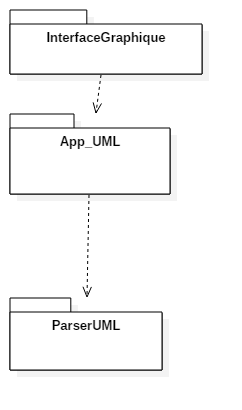
\includegraphics[scale=.3]{DiagrammePaquet.png}

Aussi nous avons divisé en plusieurs classe notre application UML.Nous avons une classe  "UML\_Classe" qui elle va contenir toute les classes du fichier UML. Ensuite cette classe possédre des opération et des attribut. les deux sont des classes qui ont chaqu'un leur propre signification. De l'autre côté on a la classe "UML\_Association" qui elle a pour unique but de démontrer les liens entre 2 classes indiqué dans le diagramme UML.
\newline
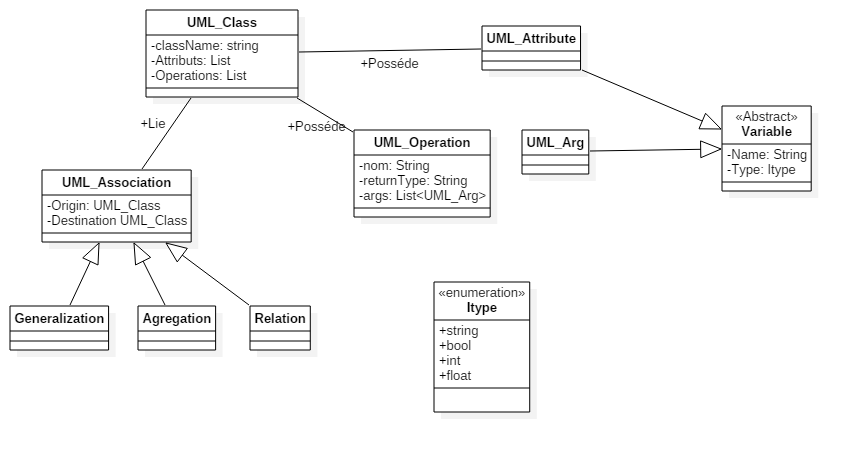
\includegraphics[scale=.4]{DiagrammeClasse.png}

\section*{Utilisation de la librairie swing}



\section*{Exécution du code java}

\end{document}
